\documentclass[10pt,a4paper,twoside]{llncs}
\usepackage[utf8]{inputenc}
\usepackage{amsmath,amsfonts,amssymb}
\usepackage{graphicx,float}
\usepackage{algorithmic,algorithm}
\usepackage{tikz}
\usetikzlibrary{matrix}
\usetikzlibrary{matrix,arrows,shapes}%,decorations.pathmorphing,snakes

\pagestyle{headings}%page numbers

%%%%%%%%%%%%%%%%%%%%%%%%%%% VERSIONES %%%%%%%%%%%%%%%%%%%%%%%%%%%%%%%%%%%%%%%%%
%%%% This file is generated by Makefile.
%%% Do not edit this file!
%%%
	\gdef\GITAbrHash{74b8017}	\gdef\GITAuthorDate{Sat Sep 15 21:59:40 2012 +0200}	\gdef\GITAuthorName{srgblnch}
%\newcommand{\version}{git: \GITAuthorDate \; (revision~\GITAbrHash)}

\usepackage{gitinfo}
\newcommand{\version}{github.Papers: \gitCommitterDate\;(revision \gitAbbrevHash) }
%%%%%%%%%%%%%%%%%%%%%%%%%%%%%%%%%%%%%%%%%%%%%%%%%%%%%%%%%%%%%%%%%%%%%%%%%%%%%%%

\title{Generalised Rijndael}
\author{Sergi Blanch-Torn\'e\inst{1}, Ramiro Moreno Chiral\inst{2}, Francesc Seb\'e Feixa\inst{2}}
 \institute{
 Escola Polit\`ecnica Superior, Universitat de Lleida. Spain.\\
 \email{\tt sblanch@alumnes.udl.es}
 \and 
 Departament de Matem\`atica. Universitat de Lleida. Spain.\\
 \email{\tt \{ramiro,fsebe\}@matematica.udl.es}
 }

%%% abreviaturas matem\'aticas
% Enteros
\newcommand{\Z}{\ensuremath{\mathbb{Z}}} 

% Anillo de los enteros mod n
\newcommand{\Zn}[1]{\ensuremath{\mathbb{Z}/#1\mathbb{Z}}} 

% Cuerpo finito de orden p (primo)
\newcommand{\Fq}[1]{\ensuremath{\mathbb{F}_#1}} 

% Cuerpo finito de caractar\'{\i}stica p, grado n
\newcommand{\Fpn}[2]{\ensuremath{\mathbb{F}_{#1^#2}}} 

% Anillo polynomial con coeficientes en un cuerpo polynomial binario
\newcommand{\Fpnm}[2]{\ensuremath{\frac{\Fpn{2}{#1}[#2]}{m(#2)}}}

\renewcommand{\algorithmicrequire}{\textbf{INPUT:}}%
\renewcommand{\algorithmicensure}{\textbf{OUTPUT:}}%
\renewcommand{\algorithmiccomment}[1]{/* #1 */}%	

%used for schemas (in Matrix)
\newcommand{\myunit}{1 cm}
\tikzset{
    node style sp/.style={draw,circle,minimum size=\myunit},
    node style ge/.style={circle,minimum size=\myunit},
    arrow style mul/.style={draw,sloped,midway,fill=white},
    arrow style plus/.style={midway,sloped,fill=white},
}

\floatname{algorithm}{Algorithm}%
\floatname{definition}{Definition}%

\begin{document}
\maketitle
\begin{center}
 \today\\
 \version
\end{center}

\begin{abstract}\footnote{Partially founded by the Spanish project MTM20\_\_-\_\_\_\_\_-\_\_\_-\_\_}
 Here will be the abstract
% TODO this article comes from a real request, for small block cipher, but the tuneable parameters in rijndael creates the idea to, further than an small version, it can be generalized
\\\\    
{\bf Keywords:} Cryptography, Symmetric, Rijndael
\end{abstract}

%%%%%%%%%%%%%%%%%%%%%%%%%%%%%%%%%%%%%%%%%%%%%%%%%%%%%%%%%%%%%%%%%%%%%%%%%%%%%%%
\section{Introduction}\label{sec:intro}
% TODO There are many other options of symmetric ciphers with different block sizes. AES is very static, but rijndael allows to play with parameters. AESwrap (rfc3394) can be mention as another possibility.
\begin{itemize}
 \item \texttt{TODO:} Short view on the symmetric algorithms history
 \begin{itemize}
  \item Previous to AES was the \emph{Data Encryption Standard}, 56 bit key length and 64 bit block size, as the standard but together with other block ciphers in 64 bit block and key length.
 \end{itemize}
 \item \texttt{TODO:} Review on the AES contest
 \begin{itemize}
  \item 1997 NIST announce that is seeking a replacement for the DES.
  \item 15 ``opponents'' (plus 10 rejected due to security or efficiency reasons) 
  \item From the proposal on 1998 \cite{Daemen98aesproposal:}, \cite{Daemen:1998:BCR:646692.759487} and the revision \cite{Daemen01aes-ammended}, passing by the decision in 2000 of Rijndael chosen \cite{AES-FIPS}.
  \item and the \cite{Daemen:2002:DR:560131} book
 \end{itemize}
 \item \texttt{TODO:} About the future of the aes with the AESwrap (rfc3394) \cite{rfc3394}
\end{itemize}

% TODO problem approach (rijndael scalability)
\begin{itemize}
 \item \texttt{TODO:} rijndael scalability. As mentioned in \cite{Daemen01aes-ammended} the standard for the AES has only 3 key sizes (128,192,256 bits), but the original specification supports blocks and keys also of lengths 160 and 224 bits. In section 12.1 the extendibility of the Rijndael is set to any multiple of 4 bytes (32 bits), with a minimum of 16 bytes (the 128 bits), but why?
\end{itemize}

% TODO alternative cryptosystems
\begin{itemize}
 \item \texttt{TODO:} alternative symmetric cryptosystems. Apart than the opponents in the AES contest, thinking more in the smaller block size or, even better, variable block size.
\end{itemize}

%%%%%%%%%%%%%%%%%%%%%%%%%%%%%%%%%%%%%%%%%%%%%%%%%%%%%%%%%%%%%%%%%%%%%%%%%%%%%%%
\section{Approach to the Rijndael Schema}\label{sec:approach}
% what is a PRP? 
\begin{definition}\label{def:PRP}
 A Pseudo-Random Permutation (PRP) is defined as a application from the message space $\mathcal{M}$ and the key space $\mathcal{K}$ to the cipher space $\mathcal{C}$:
 \begin{center}
  \begin{tabular}{llll}
   PRP: & $\mathcal{M} \times \mathcal{K}$ & $\rightarrow$ & $\mathcal{C}$ \\
  \end{tabular}
 \end{center}
 such that:
 \begin{enumerate}
  \item $\exists$ ``efficient'' \emph{deterministic} algorithm $c=E(k,m)$
  \item The functions $E$ is bijective
  \item $\exists$ ``efficient'' inversion algorithm such that $m=D(k,c)$
 \end{enumerate}
\end{definition}

A pseudo-random permutation is used as a symmetric cryptosystem like Shannon have defined in \cite{shannon-comTheorySecSys}. Also Shannon have defined the concept of the \emph{perfect secrecy}
\begin{definition}\label{def:shannonPerfectSecrecy}
 A \emph{cipher} has \emph{perfect secrecy} if $\forall m_1, m_2 \in \mathcal{M} \;s.t.\; \left| m_1 \right| = \left| m_2 \right| \wedge \forall c \in \mathcal{C}$ and  $k\in_R\mathcal{K}$ (random and uniform distributed), the probability to that $c$ comes from $m_1$ or $m_2$ are the same
 \begin{center}
  $Pr[E(k,m_1)=c] = Pr[E(k,m_2)=c]$
 \end{center}
\end{definition}

This means that $c$ does not reveal \emph{any} information about the original $m$. This can also by says like: The distribution of the cipher of a message is the same than the distribution from another message, or formally:
\begin{definition}
 For a perfect secrecy system, the distributions of the ciphers between messages in the cipher space is \emph{computationally indistinguishable}\footnote{Denoted the meaning of computationally indistinguishable by the symbol $\approx_p$ because cannot be distinguished in a \emph{polynomial time}}:
 \begin{center}
  $\{ E(k,m_1) \} \approx_p \{ E(k,m_2) \} $
 \end{center}
\end{definition}

Consider an scenario where an adversary has access to a random oracle where the output of this oracle can be or the output of the PRP or a truly random output, the advantage of the adversary to distinguish between if the output is get from one or the other can be described as:
\begin{equation}\label{eq:prpAdv}
 {Adv}_{F}^{prp}(A) = Pr[{Exp}_{F}^{prp-1}(A)=1]-Pr[{Exp}_{F}^{prp-0}(A)=1]
\end{equation}
where ${Exp}_{F}^{PRP-1}$ is the probability to the adversary to win the bet that the output comes from a the PRP and ${Exp}_{F}^{PRP-0}$ when the output comes from a truly random.

\begin{definition}\label{def:securePRP}
 A PRP is secure if for all ``efficient'' adversary, the advantage to distinguish if the output is from the PRP or the truly random is ``negligible''
\end{definition}

In other words, a \emph{PRP} is secure if the permutation given by it is indistinguishable from a truly random permutation. That means an Adversary can not take any advantage from the cipher text.

% and why is Rijndael a secure PRP? FIXME: is this enough? Can explain deep from where the 2^64 comes from?
In the case of the Rijndael, the most efficient attacks on this symmetric cryptosystem, like the best key recovery attack it is \emph{only} $4$ times better than the exhaustive search using the biclique cryptoanalysis \cite{biclique-fullaes}. But this $4$ times means that we must think in aes-128 to be like an aes-126 and this is still far, far away to an efficient break because it must be down to an attack in the order of $2^{64}$. It means that this algorithm can be trusted as \emph{still secure}.

In the case of the key sizes $192$ and $256$ of the aes, and due to a weakness on the design of the key expansion, but this will be explained in section \ref{sec:keyExpansion}.

% TODO rijndael good characteristics
\begin{itemize}
 \item \texttt{TODO:} What gives to Rijndael the good characteristics that it has?
\end{itemize}

% structure of the input (fix block size)
Out of the standard specification \cite{AES-FIPS}, the revision of 1999 of the Rijndael block cipher \cite{Daemen01aes-ammended} includes the section 12 about extensions. Is in this section where are mention block and key sizes different than the standardised having steps of 32 bits in between the 3 in the standard. This extensions can be because it only changes the number of columns. It already happens with the cases where the key have more columns than the block, and in a very similar way the block can also saw it number of columns increased.

From the 4 basic operations of the Rijndael this change is the one than can need less modifications in the bases. Following what has been mention about the simplicity, and the mathematical beauty and elegance of this schema, the increase of the number of columns is the parameter that causes less modifications in the design. Let see the design in more detail in next section \ref{sec:design}.

% TODO format preserving encryption alternative?

%%%%%%%%%%%%%%%%%%%%%%%%%%%%%%%%%%%%%%%%%%%%%%%%%%%%%%%%%%%%%%%%%%%%%%%%%%%%%%%
\subsection{Design}\label{sec:design}
% TODO what is the state matrix
% TODO describe the transformations from the Shannon ``confusion and diffusion'' point of view.
\begin{itemize}
 \item \texttt{TODO:} what is in the state matrix?
 \item \texttt{TODO:} Shannon: confusion \& diffusion $\Rightarrow$ substitution \& permutation \cite{shannon-comTheorySecSys} (a bit deep than what have said in the PRP, definition \ref{def:shannonPerfectSecrecy} about perfect secrecy.
 \item \texttt{TODO:} Explain the round transformation as one (composed) operation to provide diffusion and guarantee non-linear distribution.
\end{itemize}

%%%%%%%%%%%%%%%%%%%%%%%%%%%%%%%%%%%%%%%%%%%%%%%%%%%%%%%%%%%%%%%%%%%%%%%%%%%%%%%
\section{Generalising the schema}\label{sec:generalising}

% Draw the procedure as diagram FIXME: maybe better draw using TikZ
\begin{figure}[h!]
 \centering
 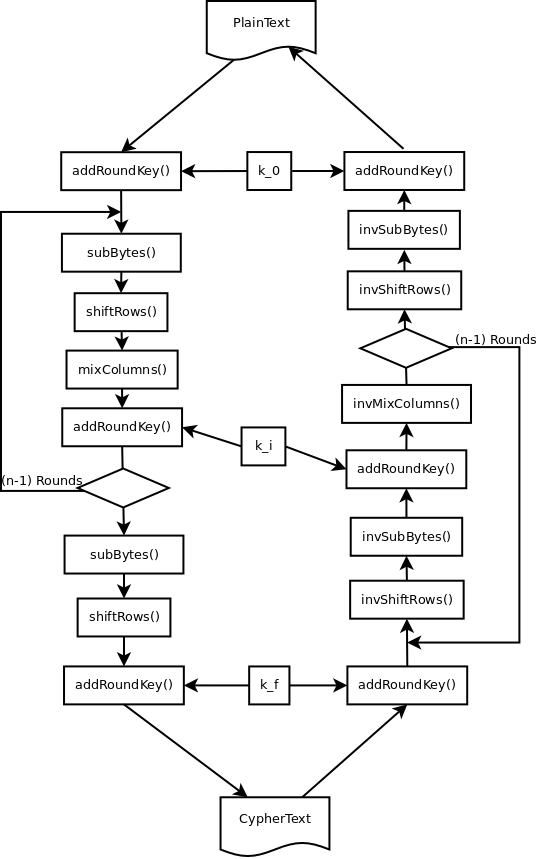
\includegraphics[scale=0.3,keepaspectratio=true]{./images/rijndaelDiagram.png}
 % rijndaelDiagram.png: 521x887 pixel, 72dpi, 18.38x31.29 cm, bb=0 0 521 887
 \caption{rijndael diagram}
 \label{fig:RijndaelDiagram}
\end{figure}
% TODO: describe

%%%%%%%%%%%%%%%%%%%%%%%%%%%%%%%%%%%%%%%%%%%%%%%%%%%%%%%%%%%%%%%%%%%%%%%%%%%%%%%
\subsection{key expansion}\label{sec:keyExpansion}
% define s Pseudo-Random Generator (PRG), What a Pseudo-Random Generator is?
The first important operation in the \emph{Rijndael} schema is the \emph{key expansion}. This operation takes the key as a seed to expand it until generate all the subkeys used on each round. In the smaller case of \emph{AES} standard, the 128 bits become expanded to 1280 extra bits to be used like if the key was this size. But why the usage 128 bits in the key, can be trusted like having an independent key 10 times longer? This important mathematical item where this security rest is what is called \emph{Pseudo-Random Generator}, PRG, generating a unique, and always the same, stream of bits from a much shorter seed. Lets define what PRG means:

\begin{definition}\label{def:PRG}
 A \emph{Pseudo-Random Generator} is a function that takes a seed and generates a much larger stream:
 \begin{center}
  \begin{tabular}{llllr}
   PRG: & $\{0,1\}^{s}$ & $\rightarrow$ & $\{0,1\}^n$ & ,where $n \ggg s$\\
  \end{tabular}
 \end{center}
 
\end{definition}
The goal is that the \emph{PRG} must be efficiently computable by a deterministic algorithm and the output of it must look random and unpredictable. In fact, this is the most important property of a \emph{PRG}, the unpredictability. But what predictability means:

\begin{definition}\label{def:unpredictability}
 Given a \emph{PRG} $G: k \rightarrow \{0,1\}^n$ is \emph{predictable} if exist an efficient algorithm \emph{A} such that:
 \begin{equation}
  \underset{k\leftarrow\mathcal{K}}{Pr}\left[A(G(k)|_{1,...,i}) = G(k)|_{i+1}\right]>\frac{1}{2}
+\epsilon \end{equation}
 for a non negligible $\epsilon$
\end{definition}

As an example, a non negligible $\epsilon$ usually is mention as a value $\geqslant\frac{1}{2^{30}}$.

The definition \ref{def:unpredictability} says that for any efficient algorithm, given to this algorithm the $i$ first bits, the probability that this algorithm predicts the next element of the stream is negligible.

The unpredictability of a \emph{PRG} is what gives to the the quality to be \emph{undistinguishable} from a \emph{pure random generator}. Even when the seed space $\mathcal{K}$ of the PRG is much smaller than the space of the output $\{0,1\}^n$.

Like in the PRP, consider an scenario where the adversary has access to a random oracle where the output of this oracle can be the output of the PRG or a truly random stream. The advantage of the adversary to distinguish from where it comes any output it has take can be described as:
\begin{equation}\label{eq:prgAdv}
 {Adv}_{prg}[A,G] = \left|
                     \underset{k\overset{R}{\leftarrow}\mathcal{K}}{Pr}\left[A(G(k))=1\right]-
                     \underset{r\overset{R}{\leftarrow}\{0,1\}^n}{Pr}\left[A(r)=1\right]
                    \right|\in [0,1]
\end{equation}
That means if the probability gets close to 1, the adversary can distinguish $G$ from random; and if it is close to 0 cannot.

\begin{definition}
 Given $G: k \rightarrow \{0,1\}^n$, is a \emph{secure PRG} if $\forall$ efficient statistical test ${Adv}_{prg}[A,G]$ is negligible.
\end{definition}

Following definition \ref{def:unpredictability} about the unpredictability, the $\epsilon$ is $\leqslant\frac{1}{2^{80}}$ to be considered as negligible.

%What can be made with the KeyExpansion() ``playing'' with the parameters (\#rows, \#columns, wordsize) from the key point of view (message things later).
\begin{algorithm}
 \caption{KeyExpansion}
 \label{alg:keyExpansion}
 \begin{algorithmic}[1]
  \REQUIRE byte k[nRows*nColumns], nRounds, nRowns, nColumns, wSize
  \ENSURE word w[nRouns*(nRows+1)]
  \STATE i := 0
  \WHILE{$i<nColumns$}
    \STATE w[i] := word($k[nRows*(i+c)$ for $c$ in $range(nColumns)]$)
  \ENDWHILE
  \STATE i := nColumns
  \WHILE{$i<nRouns*(nRows+1)$}
    \STATE temp := w[i-1]
    \IF{i mod nColumns == 0}
      \STATE temp := SubWord(RotWord(temp)) $\oplus$ Rcon[i/nColumns]
    \ELSE
      \STATE temp := SubWord(temp)
    \ENDIF
    \STATE w[i] := w[i-nColumns] $\oplus$ temp
    \STATE i++
  \ENDWHILE
 \end{algorithmic}
\end{algorithm}

Back to the \emph{key expansion} of the \emph{Rijndael}, and assuming that it is a \emph{secure PRG}, it is time to take a look on the algorithm itself to ``read'' what can be generalized because this is the purpose of this paper. The input of the algorithm \ref{alg:keyExpansion}\footnote{This algorithm has been taken from the version 2 of the AES proposal \cite{Daemen01aes-ammended} that is the same than becomes the NIST standard \cite{AES-FIPS}. But is different than the book from the Rijndael authors \cite{Daemen:2002:DR:560131}, published later than the standard} takes, further than the seed key, the number of \emph{rounds}, the number of \emph{rows} and \emph{columns}, and also the \emph{word size}.
%TODO: check how it was the keyExpansion in the first proposal \cite{Daemen98aesproposal:}

All those parameters are necessary to have in the output an expanded key large enough to use all the necessary subparts under each round, as it is shown in the figure \ref{fig:RijndaelDiagram}.

% draw the algorithm as a diagram
\begin{figure}[h!]
\begin{center}
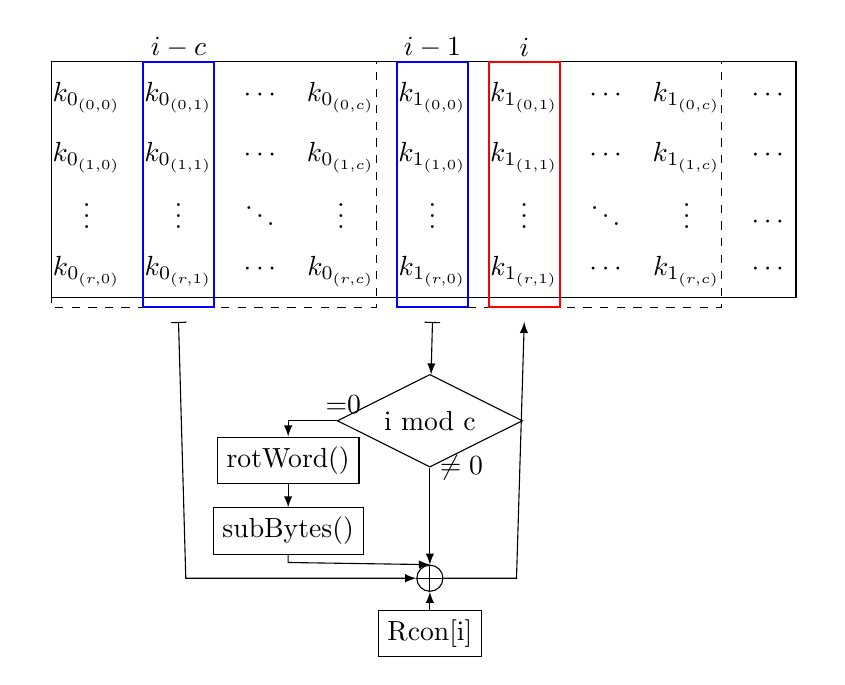
\begin{tikzpicture}[>=latex]
\matrix (k) [matrix of math nodes,nodes = {node style ge},%
              %left delimiter  = (,right delimiter = ),
              column sep=-0.1cm,row sep=-0.5cm,
             ] at (0,0)
        {
          k_{0_{(0,0)}} & k_{0_{(0,1)}} & \cdots & k_{0_{(0,c)}} &
          k_{1_{(0,0)}} & k_{1_{(0,1)}} & \cdots & k_{1_{(0,c)}} &
          \cdots \\%&
          %k_{n_{(0,0)}} & k_{n_{(0,1)}} & \cdots & k_{n_{(0,c)}} \\
          k_{0_{(1,0)}} & k_{0_{(1,1)}} & \cdots & k_{0_{(1,c)}} &
          k_{1_{(1,0)}} & k_{1_{(1,1)}} & \cdots & k_{1_{(1,c)}} &
          \cdots \\%&
          %k_{n_{(1,0)}} & k_{n_{(1,1)}} & \cdots & k_{n_{(1,c)}} \\
          \vdots        & \vdots        & \ddots & \vdots        &
          \vdots        & \vdots        & \ddots & \vdots        &
          \cdots        \\%&
          %\vdots        & \vdots        & \ddots & \vdots        \\
          k_{0_{(r,0)}} & k_{0_{(r,1)}} & \cdots & k_{0_{(r,c)}} &
          k_{1_{(r,0)}} & k_{1_{(r,1)}} & \cdots & k_{1_{(r,c)}} &
          \cdots \\%&
          %k_{n_{(r,0)}} & k_{n_{(r,1)}} & \cdots & k_{n_{(r,c)}}\\
        };
\draw [] (k-1-1.north west) rectangle (k-4-9.south east);
\draw [dashed] (k-1-1.north west) rectangle (k-4-4.south east);
\draw [dashed] (k-1-5.north west) rectangle (k-4-8.south east);
%\draw [dashed] (k-1-10.north west) rectangle (k-4-13.south east);

%boxes to get the necessary columns
\draw [blue,thick] (k-1-2.north west) rectangle (k-4-2.south east);
\draw [blue,thick] (k-1-5.north west) rectangle (k-4-5.south east);
\draw [red,thick] (k-1-6.north west) rectangle (k-4-6.south east);
% 
\node [diamond,draw,aspect=2] (imodc) at (.1,-3) {i mod c};
\node [rectangle,draw] (rotWord) at (-1.7,-3.5) {rotWord()};
\node [rectangle,draw] (subBytes) at (-1.7,-4.4) {subBytes()};
\node [circle,draw] (xor) at (.1,-5) {};
 \draw [-] (xor.north) -- (xor.south);
 \draw [-] (xor.west) -- (xor.east);
\node [rectangle,draw] (rcon) at (.1,-5.7) {Rcon[i]};
\node [] (eq0) at (-1,-2.8) {=0};
\node [] (neq) at (.5,-3.6) {$\neq0$};
\node [] (neq) at (k-1-2.north) {$i-c$};
\node [] (neq) at (k-1-5.north) {$i-1$};
\node [] (neq) at (k-1-6.north) {$i$};
% 
% %arrows to set into the algorithm
\draw [|->] (k-4-2.south) -- (-3,-5) -- (xor.west);
%\draw [|->] (k-4-5.south) -- (-.94,-2) -- (-1.5,-2) -- (imodc);
\draw [|->] (k-4-5.south) -- (imodc);
\draw [->] (imodc.west) -- (-1.7,-3) -- (rotWord.north);
\draw [->] (rotWord.south) -- (subBytes.north);
\draw [->] (imodc.south) -- (xor.north);
\draw [->] (subBytes.south) -- (-1.7,-4.8) -- (xor.north);
\draw [->] (xor.east) -- (1.2,-5) -- (k-4-6.south);
\draw [->] (rcon.north)--(xor.south);

\end{tikzpicture}
\caption{Block diagram of the iterative construction of the \emph{Rijndael Key Expansion} as a \emph{PseudoRandomGenerator}, PRG}
\label{fig:keyExpansionDiagram}
\end{center}
\end{figure}

Perhaps a better way to see the algorithm \ref{alg:keyExpansion} is the figure \ref{fig:keyExpansionDiagram}. From steps 1 to 5 in the algorithm it simply ``moves'' the input key to the first part of the generated output. The main part of the algorithm, starts on the step 6 where each column further than the original columns of the key are generated.

With this figure seems to be easier to recognise this iterative algorithm, that is generating the new column $i$ by taking the previous (with may be some transformations when the key size is bigger than the block size) and the one in the same relative position of the previous \emph{subkey}, to do over it some transformations to introduce diffusion and confusion in the newer bits generation.

Each step finish with 3 \emph{xor} operations to catch together all the partials on this step generation. The \emph{xor} operation is the most important operation and is the most used in the lower level of the \emph{Rijndael}. This is one of the bests characteristics of this algorithm.

\begin{itemize}
 \item \texttt{TODO:} subBytes() is used here (then the SBox) but will be explained deeper in section \ref{sec:subBytes}.
 \item \texttt{TODO:} What means to have different number of columns in the message than in the key matrix representation.
 \item \texttt{TODO:} Explain what is the proposal of the Rcon matrix (or as a recursive function).
\end{itemize}

% weakness in the key expansion of rijndael when key size != block size
An attack to the \emph{PRG} of the Rijndael is described in \cite{fullaes-192-256} and affects the cases where the size of the key is not the same than the size of the block. Even that, this attack requires up to $2^{99}$ pairs $(m,c)$ and $4$ \emph{related keys}\footnote{\emph{Related keys} means that the \emph{Hamming} distances are very short and the difference between one key to another are a few bits that are flipped.}. The recover time of this attack is around $2^{99}$ that is still far away from a weakness to be worried to untrust the algorithm. Also avoiding to use related keys, this attack would not apply.
%FIXME:it may would be developed or rewritten better
%FIXME: check better this article \cite{fullaes-192-256} to review if it have relation with use the number of columns of the block size instead of the key size.

%%%%%%%%%%%%%%%%%%%%%%%%%%%%%%%%%%%%%%%%%%%%%%%%%%%%%%%%%%%%%%%%%%%%%%%%%%%%%%%
\subsection{Rounds}\label{sec:rounds}
% TODO why n rounds and not more, not less?

In the AES proposal of the Rijndael \cite{Daemen01aes-ammended} (section 4.1) the number of rounds is described as a function of the block and the key length, followed by the table:
\begin{equation}\label{tab:nrounds}
%\begin{center}
\begin{tabular}{|c||c|c|c|}
\hline
$N_r$     & $N_b = 4$ & $N_b = 6$ & $N_b = 8$ \\ \hline\hline
$N_k = 4$ &    $10$   &    $12$   &    $14$   \\ \hline
$N_k = 6$ &    $12$   &    $12$   &    $14$   \\ \hline
$N_k = 8$ &    $14$   &    $14$   &    $14$   \\ \hline
\end{tabular}
%\end{center}
\end{equation}

 But is in section 7.6 where is said that this number has been determined by looking in to the most efficient attacks (known at that time) and adding a security margin. That is improved with in section 12.1, where the number of rounds is described by a function:
\begin{equation}\label{eq:nrounds}
 N_r = max(N_k,N_b)+6
\end{equation}
This function means that the number of rounds is the biggest number of columns between the block and the key, plus the security margin set as $6$.

\begin{itemize}
 \item \texttt{TODO:} But, with this, there isn't a proof of why those sizes yet.
\end{itemize}



%%%%%%%%%%%%%%%%%%%%%%%%%%%%%%%%%%%%%%%%%%%%%%%%%%%%%%%%%%%%%%%%%%%%%%%%%%%%%%%
\subsection{subBytes}\label{sec:subBytes}
This transformation is a non-linear substitution of each word in the \emph{state} matrix. In the original Rijndael it is used a substitution table called \emph{S-Box}. This S-Box is represented in the figure \ref{tab:sbox8} and there is also an inverse of it in figure \ref{tab:inv-sbox8}.

\begin{figure}[h!]{\tiny
\begin{center}
\begin{tabular}[]{|l||r|r|r|r|r|r|r|r|r|r|r|r|r|r|r|r|}\hline
    & 0x0 &0x1 &0x2 &0x3 &0x4 &0x5 &0x6 &0x7 &0x8 &0x9 &0xA &0xB &0xC &0xD &0xE &0xF \\\hline\hline
0x0 & 0x63&0x7C&0x77&0x7B&0xF2&0x6B&0x6F&0xC5&0x30&0x01&0x67&0x2B&0xFE&0xD7&0xAB&0x76\\\hline
0x1 & 0xCA&0x82&0xC9&0x7D&0xFA&0x59&0x47&0xF0&0xAD&0xD4&0xA2&0xAF&0x9C&0xA4&0x72&0xC0 \\\hline
0x2 & 0xB7&0xFD&0x93&0x26&0x36&0x3F&0xF7&0xCC&0x34&0xA5&0xE5&0xF1&0x71&0xD8&0x31&0x15 \\\hline
0x3 & 0x04&0xC7&0x23&0xC3&0x18&0x96&0x05&0x9A&0x07&0x12&0x80&0xE2&0xEB&0x27&0xB2&0x75 \\\hline
0x4 & 0x09&0x83&0x2C&0x1A&0x1B&0x6E&0x5A&0xA0&0x52&0x3B&0xD6&0xB3&0x29&0xE3&0x2F&0x84 \\\hline
0x5 & 0x53&0xD1&0x00&0xED&0x20&0xFC&0xB1&0x5B&0x6A&0xCB&0xBE&0x39&0x4A&0x4C&0x58&0xCF \\\hline
0x6 & 0xD0&0xEF&0xAA&0xFB&0x43&0x4D&0x33&0x85&0x45&0xF9&0x02&0x7F&0x50&0x3C&0x9F&0xA8 \\\hline
0x7 & 0x51&0xA3&0x40&0x8F&0x92&0x9D&0x38&0xF5&0xBC&0xB6&0xDA&0x21&0x10&0xFF&0xF3&0xD2 \\\hline
0x8 & 0xCD&0x0C&0x13&0xEC&0x5F&0x97&0x44&0x17&0xC4&0xA7&0x7E&0x3D&0x64&0x5D&0x19&0x73 \\\hline
0x9 & 0x60&0x81&0x4F&0xDC&0x22&0x2A&0x90&0x88&0x46&0xEE&0xB8&0x14&0xDE&0x5E&0x0B&0xDB \\\hline
0xA & 0xE0&0x32&0x3A&0x0A&0x49&0x06&0x24&0x5C&0xC2&0xD3&0xAC&0x62&0x91&0x95&0xE4&0x79 \\\hline
0xB & 0xE7&0xC8&0x37&0x6D&0x8D&0xD5&0x4E&0xA9&0x6C&0x56&0xF4&0xEA&0x65&0x7A&0xAE&0x08 \\\hline
0xC & 0xBA&0x78&0x25&0x2E&0x1C&0xA6&0xB4&0xC6&0xE8&0xDD&0x74&0x1F&0x4B&0xBD&0x8B&0x8A \\\hline
0xD & 0x70&0x3E&0xB5&0x66&0x48&0x03&0xF6&0x0E&0x61&0x35&0x57&0xB9&0x86&0xC1&0x1D&0x9E \\\hline
0xE & 0xE1&0xF8&0x98&0x11&0x69&0xD9&0x8E&0x94&0x9B&0x1E&0x87&0xE9&0xCE&0x55&0x28&0xDF \\\hline
0xF & 0x8C&0xA1&0x89&0x0D&0xBF&0xE6&0x42&0x68&0x41&0x99&0x2D&0x0F&0xB0&0x54&0xBB&0x16 \\\hline
\end{tabular}
\end{center}}
\caption{Sbox for 8 bits word size}
\label{tab:sbox8}
\end{figure}

\begin{figure}[h!]{\tiny
\begin{center}
\begin{tabular}[]{|l||r|r|r|r|r|r|r|r|r|r|r|r|r|r|r|r|}\hline
    & 0x0& 0x1& 0x2& 0x3& 0x4& 0x5& 0x6& 0x7& 0x8& 0x9& 0xA& 0xB& 0xC& 0xD& 0xE& 0xF\\\hline\hline
0x0 &0x52&0x09&0x6A&0xD5&0x30&0x36&0xA5&0x38&0xBF&0x40&0xA3&0x9E&0x81&0xF3&0xD7&0xFB\\\hline
0x1 &0x7C&0xE3&0x39&0x82&0x9B&0x2F&0xFF&0x87&0x34&0x8E&0x43&0x44&0xC4&0xDE&0xE9&0xCB\\\hline
0x2 &0x54&0x7B&0x94&0x32&0xA6&0xC2&0x23&0x3D&0xEE&0x4C&0x95&0x0B&0x42&0xFA&0xC3&0x4E\\\hline
0x3 &0x08&0x2E&0xA1&0x66&0x28&0xD9&0x24&0xB2&0x76&0x5B&0xA2&0x49&0x6D&0x8B&0xD1&0x25\\\hline
0x4 &0x72&0xF8&0xF6&0x64&0x86&0x68&0x98&0x16&0xD4&0xA4&0x5C&0xCC&0x5D&0x65&0xB6&0x92\\\hline
0x5 &0x6C&0x70&0x48&0x50&0xFD&0xED&0xB9&0xDA&0x5E&0x15&0x46&0x57&0xA7&0x8D&0x9D&0x84\\\hline
0x6 &0x90&0xD8&0xAB&0x00&0x8C&0xBC&0xD3&0x0A&0xF7&0xE4&0x58&0x05&0xB8&0xB3&0x45&0x06\\\hline
0x7 &0xD0&0x2C&0x1E&0x8F&0xCA&0x3F&0x0F&0x02&0xC1&0xAF&0xBD&0x03&0x01&0x13&0x8A&0x6B\\\hline
0x8 &0x3A&0x91&0x11&0x41&0x4F&0x67&0xDC&0xEA&0x97&0xF2&0xCF&0xCE&0xF0&0xB4&0xE6&0x73\\\hline
0x9 &0x96&0xAC&0x74&0x22&0xE7&0xAD&0x35&0x85&0xE2&0xF9&0x37&0xE8&0x1C&0x75&0xDF&0x6E\\\hline
0xA &0x47&0xF1&0x1A&0x71&0x1D&0x29&0xC5&0x89&0x6F&0xB7&0x62&0x0E&0xAA&0x18&0xBE&0x1B\\\hline
0xB &0xFC&0x56&0x3E&0x4B&0xC6&0xD2&0x79&0x20&0x9A&0xDB&0xC0&0xFE&0x78&0xCD&0x5A&0xF4\\\hline
0xC &0x1F&0xDD&0xA8&0x33&0x88&0x07&0xC7&0x31&0xB1&0x12&0x10&0x59&0x27&0x80&0xEC&0x5F\\\hline
0xD &0x60&0x51&0x7F&0xA9&0x19&0xB5&0x4A&0x0D&0x2D&0xE5&0x7A&0x9F&0x93&0xC9&0x9C&0xEF\\\hline
0xE &0xA0&0xE0&0x3B&0x4D&0xAE&0x2A&0xF5&0xB0&0xC8&0xEB&0xBB&0x3C&0x83&0x53&0x99&0x61\\\hline
0xF &0x17&0x2B&0x04&0x7E&0xBA&0x77&0xD6&0x26&0xE1&0x69&0x14&0x63&0x55&0x21&0x0C&0x7D\\\hline

\end{tabular}
\end{center}}
\caption{Inverse Sbox for 8 bits word size}
\label{tab:inv-sbox8}
\end{figure}

From the programmatic point of view the use of those boxes is so simple. Because the wordsize is 8 bits, by splitting the data to transform in two parts of 4 bits you can get the row and the column, taking the value in the cell as the value of the substitution. In the decipher operation, is used the inverse of the box, and with the same procedure of split the word and find the coordinates, but now with the inverse S-Box, the value you get back is the original data.

As an example, to transform the data \texttt{0x39} localise the cell in row \texttt{0x3} column \texttt{0x9}, and change the state matrix value with \texttt{0x12}. In the decipher procedure the transformation will be from the value \texttt{0x12}, reading the row \texttt{0x1} column \texttt{0x2} the cell have the value \texttt{0x39}, the original of this example. Check any other example using figures \ref{tab:sbox8} and \ref{tab:inv-sbox8} to do it and undo.

% abstraction of what it is, independent from the #rows, #columns, wordsize

But this tool of the \emph{S-Box} is a faster way to compose two transformations in one and with not much computation.

% operations in the polynomial field F_{2^w} w: wordsize
The first transformation is to compute the multiplicative inverse in the polynomial field \Fpn{2}{w}, where w is the wordsize ($w=8$ in the original Rijndael). The second transformation is an affine transformation over the polynomial field \Fpn{2}{w}. In the original Rijndael is:
\begin{equation}\label{eq:subBytes:affine}
 b_{i}' = b_{i} \oplus b_{(i+4)mod8} \oplus b_{(i+5)mod8} \oplus 
          b_{(i+6)mod8} \oplus b_{(i+7)mod8} \oplus c_{i}
\end{equation}
Where $b$ is the byte to be transformed and $c$ is a fix value \texttt{0x63=0b01100011}. This transformation can be expressed as a matrix operation:

\begin{equation}
 \left[
  \begin{array}{c}
    b_{0}'\\b_{1}'\\b_{2}'\\b_{3}'\\b_{4}'\\b_{5}'\\b_{6}'\\b_{7}'
  \end{array}
 \right]=\left[
  \begin{array}{cccccccc}
    1&0&0&0&1&1&1&1\\
    1&1&0&0&0&1&1&1\\
    1&1&1&0&0&0&1&1\\
    1&1&1&1&0&0&0&1\\
    1&1&1&1&1&0&0&0\\
    0&1&1&1&1&1&0&0\\
    0&0&1&1&1&1&1&0\\
    0&0&0&1&1&1&1&1\\
  \end{array}
 \right]\cdot\left[
  \begin{array}{c}
    b_{0}\\b_{1}\\b_{2}\\b_{3}\\b_{4}\\b_{5}\\b_{6}\\b_{7}
  \end{array}
 \right]+\left[
  \begin{array}{c}
    1\\1\\0\\0\\0\\1\\1\\0
  \end{array}
 \right]
\end{equation}

% FIXME (review) draw schematic of this step

\begin{figure}[h!]
\begin{center}
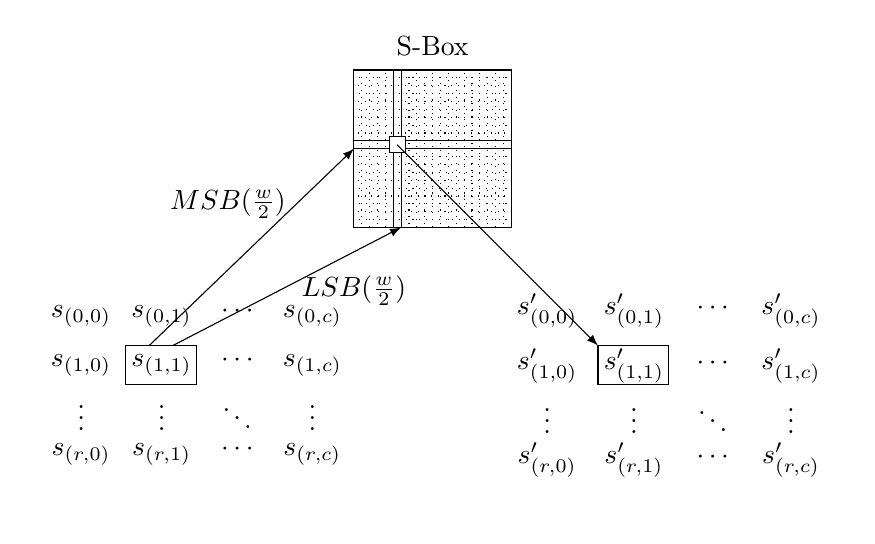
\begin{tikzpicture}[>=latex]

 \matrix (s) [matrix of math nodes,nodes = {node style ge},%
              %left delimiter  = (,right delimiter = ),
              column sep=-0.1cm,row sep=-0.5cm,
             ] at (-3,0)
        {
          s_{(0,0)} & s_{(0,1)} & \cdots & s_{(0,c)} \\
          s_{(1,0)} & s_{(1,1)} & \cdots & s_{(1,c)} \\
          \vdots    & \vdots    & \ddots & \vdots    \\
          s_{(r,0)} & s_{(r,1)} & \cdots & s_{(r,c)} \\
        };

\draw (-3.9,0.5)rectangle(-3,0);

 \matrix (s') [matrix of math nodes,nodes = {node style ge},%
              %left delimiter  = (,right delimiter = ),
              column sep=-0.1cm,row sep=-0.5cm,
             ] at (3,0)
        {
          s'_{(0,0)} & s'_{(0,1)} & \cdots & s'_{(0,c)} \\
          s'_{(1,0)} & s'_{(1,1)} & \cdots & s'_{(1,c)} \\
          \vdots    & \vdots    & \ddots & \vdots    \\
          s'_{(r,0)} & s'_{(r,1)} & \cdots & s'_{(r,c)} \\
        };
\draw (2.1,0.5)rectangle(3,0);

%sbox
\draw (-1,4)rectangle(1,2);
%x
\draw [dotted](-1,2.0)rectangle(1,2.1);
\draw [dotted](-1,2.2)rectangle(1,2.3);
\draw [dotted](-1,2.4)rectangle(1,2.5);
\draw [dotted](-1,2.6)rectangle(1,2.7);
\draw [dotted](-1,2.8)rectangle(1,2.9);
\draw (-1,3)rectangle(1,3.1);
\draw [dotted](-1,3.2)rectangle(1,3.3);
\draw [dotted](-1,3.4)rectangle(1,3.5);
\draw [dotted](-1,3.6)rectangle(1,3.7);
\draw [dotted](-1,3.8)rectangle(1,3.9);
%y
\draw [dotted](-.9,4)rectangle(-.8,2);
\draw [dotted](-.7,4)rectangle(-.6,2);
\draw (-.5,4)rectangle(-.4,2);
\draw [dotted](-.3,4)rectangle(-.2,2);
\draw [dotted](-.1,4)rectangle(0,2);
\draw [dotted](.1,4)rectangle(.2,2);
\draw [dotted](.3,4)rectangle(.4,2);
\draw [dotted](.5,4)rectangle(.6,2);
\draw [dotted](.7,4)rectangle(.8,2);
\draw [dotted](.9,4)rectangle(1,2);
%cell
\draw [fill=white] (-.55,2.95)rectangle(-.35,3.15);
%arrows
\draw [->] (-3.6,0.5)--(-1,3);%x
\draw [->] (-3.3,0.5)--(-.4,2);%y
\draw [->] (-.45,3.05)--(2.1,0.5);

%text
\node [rectangle] (sbox) at (0,4.3) {S-Box};
\node [rectangle] (msb) at (-2.6,2.3) {$MSB(\frac{w}{2})$};
\node [rectangle] (lsb) at (-1,1.2) {$LSB(\frac{w}{2})$};

\end{tikzpicture}
\caption{Schematic diagram of the subBytes() transformation}
\label{fig:subBytes}
\end{center}
\end{figure}

%%%%%%%%%%%%%%%%%%%%%%%%%%%%%%%%%%%%%%%%%%%%%%%%%%%%%%%%%%%%%%%%%%%%%%%%%%%%%%%
\subsubsection{How to build different SBoxes}\label{sec:sbox}

% TODO and how to build a new one with different parameters
Using the same \emph{wordsize} there are two different things that can be changed: the \texttt{0x63} and the product over the field of equation \ref{eq:subBytes:affine}. If the option is to use another wordsize this is the unique main parameter of the original Rijndael to set a different. With a wordsize of $4$ the operations will be defined over \Fpn{2}{4}, over $16$ the field will be \Fpn{2}{{16}}, and the subparameters of the affine transformation must also be set up.

\begin{itemize}
 \item \texttt{TODO:} how to build new ones with different parameters
\end{itemize}


%%%%%%%%%%%%%%%%%%%%%%%%%%%%%%%%%%%%%%%%%%%%%%%%%%%%%%%%%%%%%%%%%%%%%%%%%%%%%%%
\subsection{shiftColumns}\label{sec:shiftColumns}
% TODO abstraction of what it is, independent from the #rows, #columns, wordsize
\begin{itemize}
 \item \texttt{TODO:} What this means mathematically, independently to the parameters \#rows, \#columns, wordsize
\end{itemize}



% FIXME(review) draw schematic of this step
\begin{figure}[h!]
\begin{center}
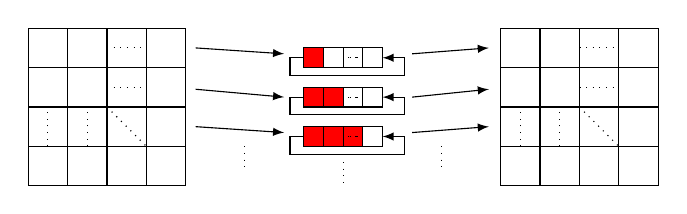
\begin{tikzpicture}[>=latex]
%input state matrix
\draw (-1.0,0.0) rectangle (1.0,0.5);%row 1
\draw (-1.0,0.5) rectangle (1.0,1.0);%row 2
\draw (-1.0,1.0) rectangle (1.0,1.5);%row ...
\draw (-1.0,1.5) rectangle (1.0,2.0);%row r
\draw (-0.5,0.0) rectangle (0.0,2.0);%c
\draw (0.5,0.0) rectangle (1.0,2.0);%c
\draw [dotted] (-0.75,0.50) -- (-0.75,1.0);
\draw [dotted] (-0.25,0.50) -- (-0.25,1.0);
\draw [dotted] (0.00,1.00) -- (0.50,0.50);
\draw [dotted] (0.00,1.25) -- (0.50,1.25);
\draw [dotted] (0.00,1.75) -- (0.50,1.75);

%first row
\draw [fill=red] (2.50,1.5) rectangle (2.75,1.75);
\draw (2.75,1.5) rectangle (3.00,1.75);
\draw (3.00,1.5) rectangle (3.25,1.75);
\draw (3.25,1.5) rectangle (3.50,1.75);
\draw [->] (2.500,1.625)--(2.325,1.625)--(2.325,1.40)--(3.775,1.40)--(3.775,1.625)--(3.50,1.625);
\draw [dotted] (3.0,1.625) rectangle (3.25,1.625);
%from to:
\draw [->](1.125,1.75)--(2.25,1.675);
\draw [->](3.875,1.675)--(4.85,1.75);

%second row
\draw [fill=red] (2.50,1.0) rectangle (2.75,1.25);
\draw [fill=red] (2.75,1.0) rectangle (3.00,1.25);
\draw (3.00,1.0) rectangle (3.25,1.25);
\draw (3.25,1.0) rectangle (3.50,1.25);
\draw [->] (2.500,1.125)--(2.325,1.125)--(2.325,0.90)--(3.775,0.90)--(3.775,1.125)--(3.50,1.125);
\draw [dotted] (3.0,1.125) rectangle (3.25,1.125);
%from to:
\draw [->](1.125,1.225)--(2.25,1.125);
\draw [->](3.875,1.125)--(4.85,1.225);

%third row
\draw [fill=red] (2.50,0.5) rectangle (2.75,0.75);
\draw [fill=red] (2.75,0.5) rectangle (3.00,0.75);
\draw [fill=red] (3.00,0.5) rectangle (3.25,0.75);
\draw (3.25,0.5) rectangle (3.50,0.75);
\draw [->] (2.500,0.625)--(2.325,0.625)--(2.325,0.40)--(3.775,0.40)--(3.775,0.625)--(3.50,0.625);
\draw [dotted] (3.00,0.625) rectangle (3.25,0.625);
%from to:
\draw [->](1.125,0.75)--(2.25,0.675);
\draw [->](3.875,0.675)--(4.85,0.75);

%vdots
\draw [dotted] (3.00,0.3) -- (3.00,0.0);
\draw [dotted] (1.75,0.5) -- (1.75,0.2);
\draw [dotted] (4.25,0.5) -- (4.25,0.2);

%output state matrix
\draw (5.0,0.0) rectangle (7.0,0.5);
\draw (5.0,0.5) rectangle (7.0,1.0);
\draw (5.0,1.0) rectangle (7.0,1.5);
\draw (5.0,1.5) rectangle (7.0,2.0);
\draw (5.5,0.0) rectangle (6.0,2.0);
\draw (6.5,0.0) rectangle (7.0,2.0);
\draw [dotted] (5.25,0.50) -- (5.25,1.0);
\draw [dotted] (5.75,0.50) -- (5.75,1.0);
\draw [dotted] (6.00,1.00) -- (6.50,0.50);
\draw [dotted] (6.00,1.25) -- (6.50,1.25);
\draw [dotted] (6.00,1.75) -- (6.50,1.75);


\end{tikzpicture}
\caption{Schematic diagram of the shiftColumns() transformation}
\label{fig:shiftColumns}
\end{center}
\end{figure}


%%%%%%%%%%%%%%%%%%%%%%%%%%%%%%%%%%%%%%%%%%%%%%%%%%%%%%%%%%%%%%%%%%%%%%%%%%%%%%%
\subsection{mixColumns}\label{sec:mixColumns}
% TODO abstraction of what it is, independent from the #rows, #columns, wordsize
% TODO polynomial ring, where the coeficients are elements from a binary polynomial field
%   \Fpnm{x}{z}, ord(m)=#rows
%   (this is, imho, one of the most important points of rijndael)
\begin{itemize}
 \item \texttt{TODO:} What this means mathematically? And what implies the changes on the parameters \#rows, \#columns, wordsize
 \item \texttt{TODO:} polynomial ring, where the coeficients are elements from a binary polynomial field \Fpnm{x}{z}, $ord(m)=\#rows$
\end{itemize}

% FIXME (review) draw schematic of this step

\begin{figure}[h!]
\begin{center}
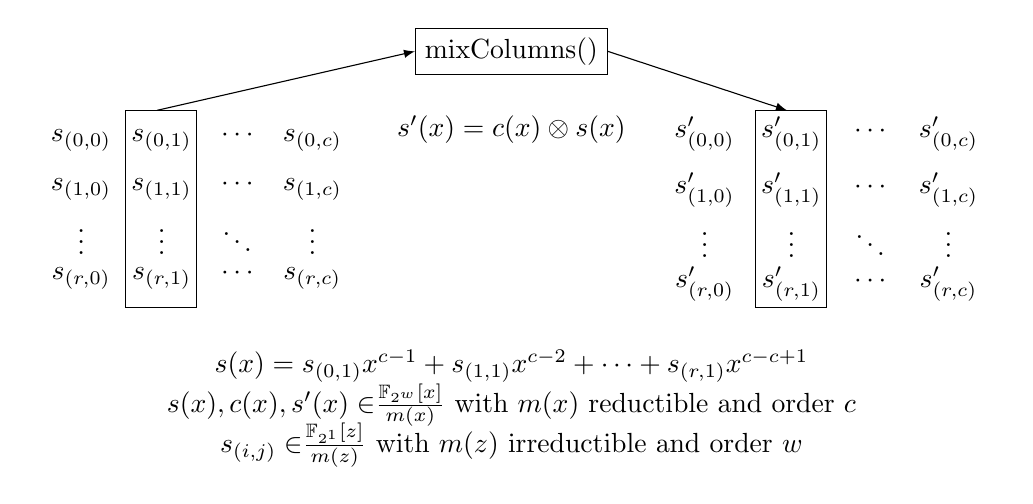
\begin{tikzpicture}[>=latex]
 
 \matrix (s) [matrix of math nodes,nodes = {node style ge},%
              %left delimiter  = (,right delimiter = ),
              column sep=-0.1cm,row sep=-0.5cm,
             ] at (-4,0)
        {
          s_{(0,0)} & s_{(0,1)} & \cdots & s_{(0,c)} \\
          s_{(1,0)} & s_{(1,1)} & \cdots & s_{(1,c)} \\
          \vdots    & \vdots    & \ddots & \vdots    \\
          s_{(r,0)} & s_{(r,1)} & \cdots & s_{(r,c)} \\
        };

\draw (-4.9,1.25)rectangle(-4,-1.25);

 \matrix (s') [matrix of math nodes,nodes = {node style ge},%
              %left delimiter  = (,right delimiter = ),
              column sep=-0.1cm,row sep=-0.5cm,
             ] at (4,0)
        {
          s'_{(0,0)} & s'_{(0,1)} & \cdots & s'_{(0,c)} \\
          s'_{(1,0)} & s'_{(1,1)} & \cdots & s'_{(1,c)} \\
          \vdots    & \vdots    & \ddots & \vdots    \\
          s'_{(r,0)} & s'_{(r,1)} & \cdots & s'_{(r,c)} \\
        };
\draw (3.1,1.25)rectangle(4,-1.25);

\node [rectangle,draw] (mixColumns) at (0,2) {mixColumns()};
 \draw [->] (-4.5,1.25)--(mixColumns.west);
 \draw [->] (mixColumns.east)--(3.5,1.25);

\node [rectangle] (poli) at (0,1.0) {$s'(x)=c(x)\otimes s(x)$};
\node [rectangle] (sx) at (0,-2) {$s(x)=s_{(0,1)}x^{c-1}+s_{(1,1)}x^{c-2}+\cdots+s_{(r,1)}x^{c-c+1}$};
\node [rectangle] (fpnm) at (0,-2.5) {$ s(x),c(x),s'(x) \in$\Fpnm{w}{x} with $m(x)$ reductible and order $c$};
\node [rectangle] (fpn) at (0,-3) {$s_{(i,j)} \in$\Fpnm{1}{z} with $m(z)$ irreductible and order $w$};

\end{tikzpicture}
\caption{Diagram of the mixColumns() operation over the polynomial ring with coeficients in a polynomial field. Invert is the same than operate with $c^{-1}(x)=d(x)$}
\label{fig:mixColumns}
\end{center}
\end{figure}

%%%%%%%%%%%%%%%%%%%%%%%%%%%%%%%%%%%%%%%%%%%%%%%%%%%%%%%%%%%%%%%%%%%%%%%%%%%%%%%
\subsection{Operate in a polynomial ring, with coeficients in a polynomial field}\label{sec:polynomialRing}
The polynomial ring used in the Rijndael schema is denoted:
$$\Fpnm{n}{x}\label{eq:polynomialRing}$$
where $m(x)$ is a composited polynomial with the same degree than the $c$ columns parameter. This describes a polynomial ring. The coefficients of this polynomial ring are elements of a polynomial field $\Fpn{2}{n}$, where this notation is a shorter of
$$\Fpn{2}{n}=\Fpnm{1}{z}\label{eq:polynomialField}$$
and in here, the polynomial $m(z)$ is an irreductible with the same degree than the wordsize ($w$). 

An improvement of the modular operations in the polynomial ring, in the specification of the rijndael schema \cite{Daemen01aes-ammended} is proposed the use of a circulant invertible matrix. In \emph{mixColumns} operation is set one fix element of the ring to be operated with each of the columns of the state matrix (in the interpretation of the column where each cell is one coefficient of this polynomial).

Then the fix polynomial element in the ring have set in the standard:
$$c(x) = (z+1)x^3+(1)x^2+(1)x+(z)$$
This is using the best notation to denote that the coefficients on the polynomial ring are elements of a polynomial field. The polynomial field have binary coefficients, then those polynomials can be shorted using a binary notation. Like $(z+1)=\texttt{0b11}=\texttt{0x3}$ and other like $(z^3+z+1)=\texttt{0b1011}=\texttt{0xB}$. Then this $c(x)$ can be shorted represented by: $c(x) = \texttt{0x3}x^3+\texttt{0x1}x^2+\texttt{0x1}x+\texttt{0x2}$. This polynomial element is coprime to the modulo ($x^4+1$) and therefore has an inverse in the ring used to revert the \emph{mixColumns}: $c^{-1}(x) = \texttt{0xB}x^3+\texttt{0xD}x^2+\texttt{0x9}x+\texttt{0xE}=d(x)$.

The matrix multiplication of this polynomial ring operation can be written as:
\begin{equation}\label{eq:MDS}
  \begin{bmatrix}
    s'_{(0,i)}\\s'_{(1,i)}\\s'_{(2,i)}\\s'_{(3,i)}
  \end{bmatrix}
  =
  \begin{bmatrix}
    z & z+1 & 1 & 1 \\
    1 & z & z+1 & 1 \\
    1 & 1 & z & z+1 \\
    z+1 & 1 & 1 & z \\
  \end{bmatrix}
  \begin{bmatrix}
    s_{(0,i)}\\s_{(1,i)}\\s_{(2,i)}\\s_{(3,i)}
  \end{bmatrix}
\end{equation}

% TODO: MaxDistanceSeparable.
% TODO: Does this circulant matrix works with $c\neq 4$?
\begin{enumerate}
 \item \texttt{TODO:} Does this circulant matrix works with $c\neq 4$?
\end{enumerate}


%%%%%%%%%%%%%%%%%%%%%%%%%%%%%%%%%%%%%%%%%%%%%%%%%%%%%%%%%%%%%%%%%%%%%%%%%%%%%%%
\subsection{addRoundKey}\label{sec:addRoundKey}
% TODO the operation where the key is used (from the 4 rijndael operations)
% TODO simply a xor operation (addition in F_2)
% TODO draw schematic of this step

\begin{figure}[h!]
\begin{center}
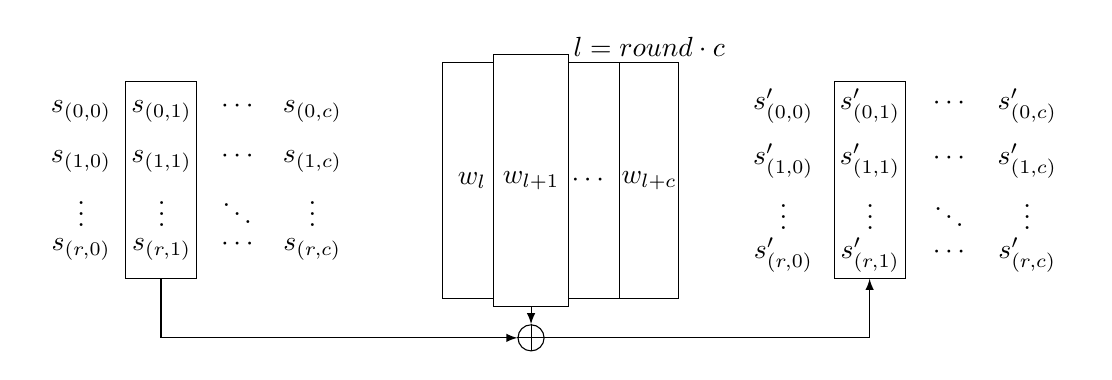
\begin{tikzpicture}[>=latex]
 
\matrix (s) [matrix of math nodes,nodes = {node style ge},%
              %left delimiter  = (,right delimiter = ),
              column sep=-0.1cm,row sep=-0.5cm,
             ] at (-5,0)
        {
          s_{(0,0)} & s_{(0,1)} & \cdots & s_{(0,c)} \\
          s_{(1,0)} & s_{(1,1)} & \cdots & s_{(1,c)} \\
          \vdots    & \vdots    & \ddots & \vdots    \\
          s_{(r,0)} & s_{(r,1)} & \cdots & s_{(r,c)} \\
        };

\draw (-5.9,1.25)rectangle(-5,-1.25);

 \matrix (s') [matrix of math nodes,nodes = {node style ge},%
              %left delimiter  = (,right delimiter = ),
              column sep=-0.1cm,row sep=-0.5cm,
             ] at (4,0)
        {
          s'_{(0,0)} & s'_{(0,1)} & \cdots & s'_{(0,c)} \\
          s'_{(1,0)} & s'_{(1,1)} & \cdots & s'_{(1,c)} \\
          \vdots    & \vdots    & \ddots & \vdots    \\
          s'_{(r,0)} & s'_{(r,1)} & \cdots & s'_{(r,c)} \\
        };
\draw (3.1,1.25)rectangle(4,-1.25);
%the central boxes of the key table
\draw        (-1.875,1.5)rectangle(-1.125,-1.5);\node [] (wl) at (-1.5,0) {$w_{l}$};
\draw        (-0.375,1.5)rectangle( 0.375,-1.5);\node [] (wld) at (0,0) {$\cdots$};
\draw        ( 0.375,1.5)rectangle( 1.125,-1.5);\node [] (wlc) at (.75,0) {$w_{l+c}$};
%the bigger column
\draw [fill=white] (-1.225,1.6)rectangle(-0.275,-1.6);\node [] (wl1) at (-.75,0) {$w_{l+1}$};
%the xor sign
\node [circle,draw] (xor) at (-.75,-2) {};
 \draw [-] (xor.north) -- (xor.south);
 \draw [-] (xor.west) -- (xor.east);
%algorithm lines
\draw [->] (-5.45,-1.25)--(-5.45,-2)--(xor.west);
\draw [->] (-.75,-1.6)--(xor.north);
\draw [->] (xor.east)--(3.55,-2)--(3.55,-1.25);

\node [] (l) at (0.75,1.7) {$l=round\cdot c$};

\end{tikzpicture}
\caption{Diagram of the addRoundKey()}%TODO}
\label{fig:addRoundKey}
\end{center}
\end{figure}


%%%%%%%%%%%%%%%%%%%%%%%%%%%%%%%%%%%%%%%%%%%%%%%%%%%%%%%%%%%%%%%%%%%%%%%%%%%%%%%
\section{Parameter combinations}\label{sec:parameterCombinations}
% TODO how, with different parameters, can have the same block sizes, and what's different between them
\begin{itemize}
 \item different parameter combinations can produce the same block (and key) sizes. What can help on the option chose?
\end{itemize}


%%%%%%%%%%%%%%%%%%%%%%%%%%%%%%%%%%%%%%%%%%%%%%%%%%%%%%%%%%%%%%%%%%%%%%%%%%%%%%%
\section{New useful sizes for Rijndael}\label{sec:newSizes}
% TODO because of the newer processors with 64 bits, it can be easy to have bigger sizes with less costs
\begin{itemize}
 \item \texttt{TODO:} With the newer architectures (64bits) which parameter changes can improve the cost of the rijndael? \cite{Daemen:1999:EBC:1267115.1267119}
\end{itemize}

%%%%%%%%%%%%%%%%%%%%%%%%%%%%%%%%%%%%%%%%%%%%%%%%%%%%%%%%%%%%%%%%%%%%%%%%%%%%%%%
%TODO: what else should be in the paper?
% \section{Attacking the schema}
% 
% \subsection{Side channel attacks}
% %?difference between precalculated sbox and rcon or compute on the fly
% % constant time operation intervals and equivalent memory use
% % key expansion calculated during the encrypt/decrypt process
% \section{Conclusions}

%%%%%%%%%%%%%%%%%%%%%%%%%%%%%%%%%%%%%%%%%%%%%%%%%%%%%%%%%%%%%%%%%%%%%%%%%%%%%%%
\bibliographystyle{ieeetr}
\bibliography{../bibtex/sblanch.bib,../bibtex/rijndael.bib,../bibtex/symmetrics.bib,../bibtex/standards.bib,../bibtex/books.bib,../bibtex/crypto.bib,../bibtex/rfc.bib}

\end{document}